\section{Sketch of approach}

\subsection{Kontextabgrenzung}
Figur \ref{fig:Kontext} zeigt das Kontextdiagramm. In der Mitte des Diagramms steht das System (blau) selbst.\\
Die ersten Überlegungen haben ergeben, dass die physikalische Umgebung eine Rolle spielen wird. Der Untergrund könnte Wasser, Erde, Stein, Stand, etc. sein und dies kann mithilfe von Sensoren ermittelt werden.\\
Außerdem sind das Wetter und die Temperatur eventuell auch zwei wichtige Komponenten. In wiefern muss der Roboter wetter beständig sein und auch hitze- und/oder kältebeständig.\\
Des Weiteren sind auf der Karte noch die Signalposten aufzufinden, die Audio-/Lichtsignale senden. Hier besteht auch eine Verbindung zum Rescue Robot, da die Signale ihn über die Karte führen.\\
Das Bergungsobjekt gehört auch in den Kontext. Der Robot soll das Bergungsobjekt mithilfe von Sensoren und einer Kamera erkennen.\\
Zudem gibt es noch einen internen und einen externen Controller. Der externe Controller ist mit dem Rescue Robot durch das Human Machine Interface (HMI) verbunden. Sobald der Robot am Bergungsobjekt angekommen ist, soll sich das HMI anschalten und der Roboterarm soll durch einen externen Controller, per Livesteuerung, gesteuert werden.\\
Die Hindernisse teilen sich auf in Wände und Objekte. Den Wänden soll der Robot ausweichen und die Objekte, welche in Abschnitt \ref{subsection:szenario} beschrieben sind, sollen bis zu einer bestimmten Größe überfahren und ab einer bestimmten Größe umfahren werden.\\
So waren die ersten Überlegungen der Gruppe zum Kontext.
\begin{figure}[htbp] 
  \centering
     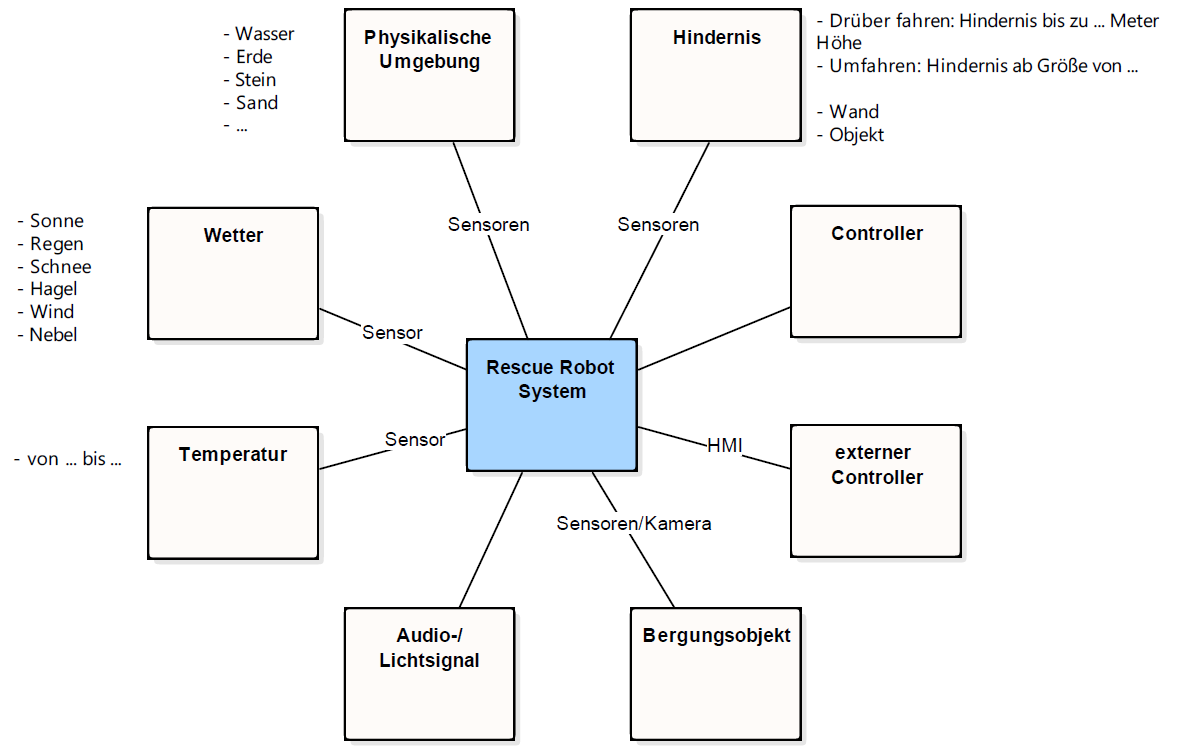
\includegraphics[width=0.5\textwidth]{Bilder/Kontextdiagramm.PNG}
  \caption{Kontextdiagramm}
  \label{fig:Kontext}
\end{figure}
\begin{flushright}
	$ [ $Katrin Glöwing$ ] $
\end{flushright}
